%File: formatting-instruction.tex
\documentclass[letterpaper]{article}
\usepackage{url,graphicx,xcolor}
\usepackage{times}
\usepackage{helvet}
\usepackage{courier}
\usepackage{hyperref}
%\usepackage[guidelines]{faikrmod3}
\usepackage[]{faikrmod3} % without guidelines
\frenchspacing
\setlength{\pdfpagewidth}{8.5in}
\setlength{\pdfpageheight}{11in}
\usepackage{float}


% THE \pdfinfo /Title AND /Author ARE NOT NECESSARY, THEY ARE METADATA FOR THE FINAL PDF FILE
\pdfinfo{
/Title (Heart Disease Risk Assessment using Bayesian Networks)
/Author (Matteo Fasulo, Luca Tedeschini, Antonio Gravina, Luca Babboni)}
\setcounter{secnumdepth}{0}  
 \begin{document}
% The file aaai.sty is the style file for AAAI Press 
% proceedings, working notes, and technical reports.
%
\title{Heart Disease Risk Assessment using Bayesian Networks}
\author{Matteo Fasulo, Luca Tedeschini, Antonio Gravina, Luca Babboni\\
Master's Degree in Artificial Intelligence, University of Bologna\\
\{ matteo.fasulo, luca.tedeschini3, antonio.gravina, luca.babboni2 \}@studio.unibo.it
}

\maketitle


\attention{DO NOT MODIFY THIS TEMPLATE - EXCEPT, OF COURSE FOR TITLE AND AUTHORS. REMOVE THE \texttt{guidelines} OPTION FROM  \texttt{$\backslash$usepackage[guidelines]\{faikrmod3\}} IN THE \LaTeX\ SOURCE IN THE FINAL VERSION.}

\begin{abstract}
\begin{quote}

\explanation{
This mini-project aims to ... \\
We use ... \\
We found that ...
}

Cardiovascular diseases (CVDs) remain the foremost global cause of mortality, claiming approximately 17.9 million lives in 2019. These diseases, which include heart attacks and strokes, accounted for 85\% of CVD-related fatalities. 
In this study, Bayesian Networks (BNs) are employed for the early detection of CVDs, with a focus on validating the predictive efficacy of various BNs and exploring the intricate interactions among diverse risk factors. Our research emphasize the importance of balancing data-driven optimization with domain knowledge for meaningful and effective CVD prediction. The study found that the BN built upon domain knowledge demonstrates remarkable predictive performance, achieving a notable ROC AUC score of 0.85, highlighting its potential for meaningful and effective CVD prediction.
\end{quote}
\end{abstract}

\section{Introduction}
\subsection{Domain}
\explanation{
Introduce your work: what you are modeling, if you are drawing inspiration from an existing model, study, paper, textbook example, challenge, \dots.\\
%
Briefly provide whatever background information on the domain you think is necessary for the reader to understand the model and your design choices.
}

In our study, we are modeling the risk of cardiovascular diseases (CVDs), a leading cause of death globally \cite{WHO2024}.
Our work draws inspiration from a paper \cite{ORDOVAS2023107405} where the authors developed a Bayesian Network (BN) to predict CVD risk by means of CVD risk factors (CVRFs) divided into modifiable and non-modifiable CVRFs.
Researchers have identified diverse CVD risk factors \cite{MAHMOOD2014999}, such as: age, sex, chest pain type, resting blood pressure, total serum cholesterol and other meaningful features.\\
Our choice of using a BN as predictive model is motivated by its ability to handle complex, real-world data and its success in healthcare applications \cite{nielsen2009bayesian}. Furthermore, BNs let us analyze how various risk factors interact, providing valuable insights into the mechanisms of CVDs.

\attention{HERE AND EVERYWHERE ELSE: ALWAYS KEEP IN MIND THAT, CRUCIALLY, WHATEVER TEXT/CODE/FIGURES/IDEAS/... YOU TAKE FROM ELSEWHERE MUST BE CLEARLY IDENTIFIED AND PROPERLY REFERENCED IN THE REPORT.}

\subsection{Aim}
\explanation{
Explain the purpose of your project: what do you intend to observe/try/experience/\dots? \\
\begin{itemize}
    \item 
Example: the purpose of this project is to implement part of the Bayesian network described in \cite{10.1371/journal.pone.0220065} and experiment with concepts seen in class \\
%
\item Another example: our aim was to experiment the effect of discretization of continuous variables \\
%
\item Yet another example: we are interested in comparing the run-time and error of approximate inference under different conditions
%
\item One final example: we studied \textit{value of information}: something mentioned in class but not covered in this module, which sparked our interest.
\end{itemize}
}

Our project aims at the creation of several BN classifiers built by using different methods, in order to predict the likelihood of CVDs based on a range of risk factors, such as the ones mentioned before. It prioritizes the maximization of the ROC AUC score, as it is proven to be particularly useful for prediction and evaluation of healthcare outcomes \cite{Marcusson}. Additionally, the project explores methods to transform continuous variables like cholesterol and heart rate into discrete categories by using established medical references, allowing the BN models to handle them more effectively. Ultimately, the project seeks to evaluate the performance of each model to get the best one in terms of results (accuracy and ROC AUC) and semantic meaningfulness.

\subsection{Method}
\explanation{
Describe the methodology you followed
\begin{itemize}
    \item 
Example: we used pgmpy library methods\footnote{This is just an example: indeed, it is NOT necessary to use pgmpy; the coding language doesn't have to be python either. Feel free to use whatever software framework suits your needs.} to implement our network and run queries. To understand if differences in models, queries, parameters or number of samples induced differences in accuracy, we varied evidence nodes, conditional probability distributions, inference method, ...
\end{itemize}
}

In order to build and test the BN classifiers, we use the `pgmpy` library and we explore different model configurations: Naive Bayes, Hill Climbing (with all its possible scoring methods, both constrained and unconstrained, provided by the library), Domain Knowledge network (using scientific literature to establish the edges) and a reduced network with feature selection. For the latter, we use a library named `PyImpetus` that implements a Markov Blanket based feature selection algorithm.
Ultimately, this aims at the identification of the BN structure and scoring method combination that maximizes the ROC AUC score for accurate heart disease prediction. This chosen model is then subjected to further analysis, regarding the structure and the properties of the network.

\subsection{Results}

\explanation{
In a few lines: what are the most noteworthy results you have observed or things you have learned/understood from this project? (only the highlights: there will be a dedicated paragraph for presenting results in the Analysis section)
}

Our exploration reveals that the structure of the BN significantly impacts performances. Although the Naive Bayes and the Hill Climbing unconstrained models yield good results, they lack semantic meaning. Conversely, the Hill Climbing constrained and the Domain Knowledge network models maintain strong explanatory power and incorporate sensible relationships between features. This highlights the importance of balancing data-driven optimization with domain knowledge to achieve a meaningful and effective BN for heart disease prediction.



\section{Model}

\explanation{
Insert a picture of your Bayesian network(s) (Figure~\ref{fig:network})
%
\begin{figure}
    \centering
    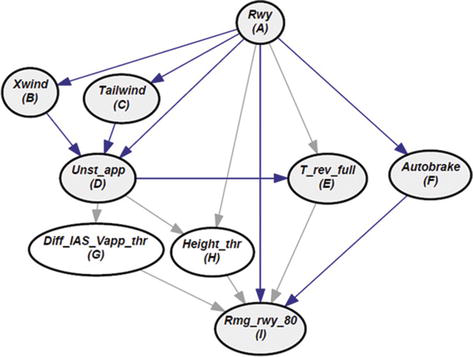
\includegraphics[scale=1.0]{F2.png}
    \caption{Bayesian network. Image taken from \url{https://www.intechopen.com/chapters/62844}}
    \label{fig:network}
\end{figure}
}

\begin{figure}
    \centering
    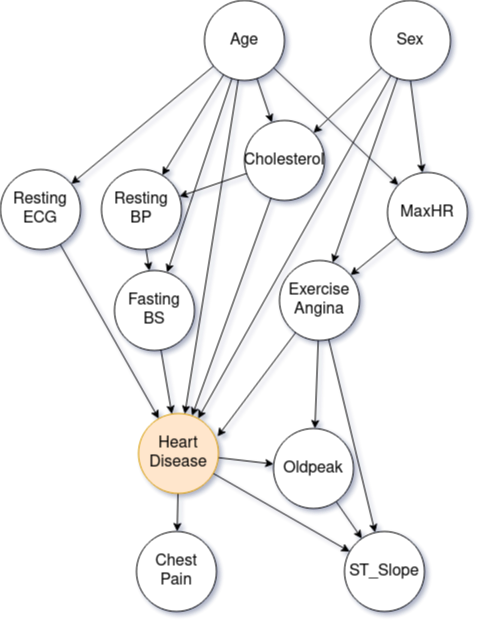
\includegraphics[scale=0.35]{latex/CVD prediction with bn.png}
    \caption{Domain Knowledge Bayesian Network structure}
    \label{fig:network}
\end{figure}

\explanation{
Explain the following aspects of your model (if there is too much to say and not enough space, put in your notebook whatever does not fit here):
\begin{itemize}
    \item nodes: if not self-explanatory, explain each random variable's meaning/intuition and type/range
    \item conditional distributions (for example, the CPTs, some or all of them)
    \item the procedure you followed to build your model (structure and conditional distributions): from reference paper? by analyzing the domain? learned from data? just assigned probability distributions arbitrarily? followed a particular methodology for building the network? ...
\end{itemize}  
In general, only write whatever is relevant and necessary to understand the rest of the report. Do not explain concepts seen in class or explained in textbooks. Do not describe models taken from textbook/literature/tutorials/libraries, like (for example) the Asia network. Instead, if you are using a model as-is: just insert a reference or URL\footnote{\url{https://www.bnlearn.com/bnrepository/}.}
}

In the BNs built for this study, each node embodies a unique random variable, each with a distinct interpretation and range. These variables include 'Age', 'Sex', 'ChestPainType', among others, all of which are pertinent to the study of CVDs. The continuous variables within the dataset have been discretized, utilizing standard ranges derived from existing scientific literature. For models that do not grasp the semantic meaning of the variables, and consequently establish links without discerning causal relationships, the Maximum Likelihood Estimator is employed to estimate the Conditional Probability Distributions (CPDs). Conversely, for the Domain Knowledge BN, the Bayesian Estimator is used.\\
For the construction of the Domain Knowledge network, we identify the causal relationships among the variables, substantiated by both scientific literature and domain knowledge. Among all the models, this particular one has been selected for the analysis of its structure and properties.
We can also consider the network with reduced dimensionality. However, it is overly simplistic and it does not take into account the majority of the features.

\section{Analysis}
\subsection{Experimental setup}
\explanation{
Briefly describe the probability queries or other experiments that you have carried out. Describe how you plan to evaluate the results (for example: are there results that you would expect?)
}

To assess the results, we employ the ROC AUC score. In order to do this, we partition the data into training ($85\%$) and testing ($15\%$) sets. Additionally, we apply KFold Cross Validation to obtain a more realistic estimate of the classifier’s performance on unseen data. The expectations are higher for the networks where we manually incorporate edges and constraints.

\subsection{Results}




\explanation{
What did you observe? \\
%
All according to expectations? \\
%
Anything surprising or worthwhile mentioning?
}
\begin{table}[H]\centering
\begin{tabular}{@{\extracolsep{1pt}}lccccc}
\\[-1.8ex]\hline 
\hline \\[-1.8ex] 
Bayesian Model    & \multicolumn{1}{c}{ROC AUC}\\
\hline\\[-1.8ex]
Naïve Bayes                 & 0.84\\ \hline\\[-1.8ex]
Hill Climbing Unconstrained & 0.86\\ \hline\\[-1.8ex]
Hill Climbing Constrained   & 0.83 \\ \hline\\[-1.8ex]
\textbf{Domain Knowledge}   & \textbf{0.85}\\ \hline\\[-1.8ex]
Reduced Network             & 0.86\\
\hline \\[-1.8ex] 
\end{tabular}
\caption{Results found for different BN construction methods}\\
\label{tab:model_res}
\end{table}

In terms of ROC AUC, all the results seem similar. However, the model that relies on domain knowledge performs slightly less effectively than both the unconstrained Hill Climbing model and the reduced network.

\section{Conclusion}
In this project, we explored various strategies for constructing a BN classifier. Our findings suggest that a fully explainable network is preferable to a high-performing network that lacks semantic meaning or does not exploit all the features. Even though these features may introduce some noise into the network, we believe that their inclusion is more beneficial than excluding them altogether. The final network achieved a ROC AUC score of $0.85$, which is commendable. Any attempt to further improve this score could potentially lead to overfitting on the dataset.

\section{Links to external resources}
\explanation{
Optionally, insert here:
\begin{itemize}
    \item a link to your GitHub or any other public repo where one can find your code (only if you did not submit your code on Virtuale) 
    \item a link to your dataset (only if you have used a dataset, for example, for learning network parameters or structure)
\end{itemize}
Leave this section empty if you have all your resources in Virtuale. \textbf{Do not insert code/outputs in this report}.
}
The notebook containing the project is available on \href{https://github.com/MatteoFasulo/BayesianHeartDisease}{GitHub}. Refer \cite{dataset} for the dataset.
\bigskip

\bibliographystyle{aaai}
\bibliography{faikrmod3.bib}


\attention{NOTICE: THIS REPORT'S LENGTH MUST NOT EXCEED \textbf{TWO PAGES} PLUS REFERENCES. THIS MAY MEAN THAT YOU WILL HAVE TO LEAVE OUT OF THE REPORT PART OF THE WORK YOU HAVE DONE OR OBSERVATIONS YOU HAVE. THIS IS NORMAL: THE REPORT SHOULD EMPHASIZE WHAT IS MOST SIGNIFICANT, NOTEWORTHY, AND REFER TO THE NOTEBOOK FOR ANYTHING ELSE. FOR ANY OTHER ASPECT OF YOUR WORK THAT YOU WOULD LIKE TO EMPHASIZE BUT CANNOT EXPLAIN HERE FOR LACK OF SPACE, FEEL FREE TO ADD COMMENTS IN THE NOTEBOOK.}


\end{document}